\documentclass[11pt,letterpaper]{article}
\usepackage[T1]{fontenc}
\usepackage{lmodern,microtype}
\usepackage[margin=1in]{geometry}
\usepackage{amsmath,amssymb,amsthm,mathtools}
\usepackage{booktabs,longtable,array}
\usepackage{enumitem,xcolor,hyperref,cleveref,graphicx,float,fancyhdr,setspace,titlesec}
\graphicspath{{figures/}{../figures/}}
\definecolor{KMBlue}{RGB}{31,70,110}
\definecolor{KMGray}{RGB}{85,92,101}
\hypersetup{colorlinks=true,linkcolor=KMBlue,citecolor=KMBlue,urlcolor=KMBlue,pdftitle={Endogenous Semantic-Witness Growth and External Latent-Reasoner Pilot},pdfauthor={Komorebi P.},hypertexnames=false}
\pagestyle{fancy}\fancyhf{}\fancyhead[L]{\small SRIC Block 23}\fancyhead[R]{\small Komorebi P.}\fancyfoot[C]{\thepage}\setlength{\headheight}{14pt}
\titleformat{\section}{\Large\bfseries\color{KMBlue}}{\thesection}{0.75em}{}
\titleformat{\subsection}{\large\bfseries\color{KMBlue}}{\thesubsection}{0.65em}{}
\setlist[itemize]{leftmargin=1.45em,itemsep=0.25em}\setlist[enumerate]{leftmargin=1.65em,itemsep=0.25em}\setstretch{1.05}
\newtheoremstyle{kmplain}{7pt}{7pt}{\itshape}{}{\bfseries\color{KMBlue}}{.}{0.5em}{}
\newtheoremstyle{kmdef}{7pt}{7pt}{}{}{\bfseries\color{KMBlue}}{.}{0.5em}{}
\newtheoremstyle{kmremark}{6pt}{6pt}{\small}{}{\bfseries\color{KMGray}}{.}{0.5em}{}
\theoremstyle{kmplain}\newtheorem{theorem}{Theorem}[section]\newtheorem{proposition}[theorem]{Proposition}\newtheorem{conditionaltheorem}[theorem]{Conditional Theorem}
\theoremstyle{kmdef}\newtheorem{definition}[theorem]{Definition}
\theoremstyle{kmremark}\newtheorem{warning}[theorem]{Warning}\newtheorem{remark}[theorem]{Remark}
\crefname{conditionaltheorem}{Conditional Theorem}{Conditional Theorems}
\DeclareMathOperator{\Aut}{Aut}
\newcommand{\R}{\mathbb R}\newcommand{\Ucal}{\mathcal U}\newcommand{\Gcal}{\mathcal G}\newcommand{\eps}{\varepsilon}\newcommand{\norm}[1]{\left\lVert #1\right\rVert}
\begin{document}
\hypersetup{pageanchor=false}
\begin{titlepage}
\centering\vspace*{1.0in}
{\Huge\bfseries\color{KMBlue} Endogenous Semantic-Witness Growth\par}
\vspace{0.15in}{\Large and an External Latent-Reasoner Pilot Contract\par}
\vspace{0.45in}{\large SRIC Block 23\par}
\vfill{\Large Komorebi P.\par}\vspace{0.12in}{\large Version 2.4, September 2026\par}
\vfill
\begin{minipage}{0.86\textwidth}\small
\textbf{Status.} The finite semantic-witness benchmark is complete and reproducible. The third-party Coconut adapter is source locked and protocol tested, but the external checkpoint was not available in the release environment and was not executed. No real-checkpoint interpretability finding is claimed.
\end{minipage}
\end{titlepage}
\hypersetup{pageanchor=true}
\pagenumbering{roman}
\begin{abstract}
We formalize semantic meaning for recurrent latent reasoning as a minimal causal-predictive quotient relative to a declared intervention language. A finite compiler receives trajectories, semantic-preserving twins, anonymous interventions, protected future consequences, and final answers, but no gold intermediate semantic coordinates. Across thirty-six fresh episodes it distinguishes unique identification, identification up to gauge, partial ontology, protected underidentification, and destructive information loss with all certificates correct. An answer-only quotient attains high answer accuracy but fails future and intervention sufficiency. Audit-only counterfactual packet patching supports the selected quotient and rejects answer-only, PCA, and random controls. We also release a source-locked adapter for a public multimode GPT-2 Coconut checkpoint on PrOntoQA. The adapter supports exact trace capture, replay, truncation, permutation, noise replacement, semantic-twin transplantation, and same-answer/different-proof transplantation. The external checkpoint was not present in the release environment, so the real-model track remains an execution-ready protocol rather than an empirical result.
\end{abstract}
\tableofcontents\clearpage
\pagenumbering{arabic}
\section{Endogenous Semantic-Witness Growth and External Latent-Reasoner Pilot}
\label{sec:block23}

Blocks 16 through 22 progressively removed supplied structure from the Neuralese transport problem.  They established direct causal intervention, training-generated latent repair, distribution-indexed semantic charts, chartwise cross-architecture transport, obstruction-guided transport-grammar growth, and correspondence-free transport from intervention orbits.  One central scaffold remained: the protected intermediate semantic coordinates used to judge whether a latent packet had the intended meaning were supplied by the benchmark author.

Block 23 separates two questions that must not be collapsed.  The first is theoretical and finite:
\begin{equation}
\boxed{
\begin{gathered}
\text{Can a lineage construct a minimal semantic quotient from}\\
\text{future consequences, interventions, and semantic twins}\\
\text{without receiving gold intermediate semantic coordinates?}
\end{gathered}}
\label{eq:b23-central-question}
\end{equation}
The second is empirical: can the same contract be applied to a third-party latent-reasoning checkpoint?  The released package answers the first question positively inside a controlled finite fixture and supplies a source-locked adapter for the second.  The external checkpoint was not present in the release environment and was not executed.  The two evidential statuses are recorded separately.

\subsection{Causal-predictive semantics}

Let $H$ be a measurable latent-state space, let $\Ucal$ be a declared finite intervention language, and let $Y^{u}_{0:r}$ denote the protected future observations, actions, scores, or externally checkable consequences generated after intervention word $u\in\Ucal^{\le r}$.  The semantic object sought in this block is not a linguistic paraphrase of every coordinate.  It is the quotient induced by the distinctions that matter for permitted future experiments.

\begin{definition}[Causal-predictive equivalence]
For $h,h'\in H$, write
\begin{equation}
h\sim_{\Ucal,r}h'
\end{equation}
when
\begin{equation}
\mathcal L\!\left(Y^{u}_{0:r}\mid h\right)
=
\mathcal L\!\left(Y^{u}_{0:r}\mid h'\right)
\qquad
\text{for every }u\in\Ucal^{\le r}.
\label{eq:b23-causal-equivalence}
\end{equation}
The quotient
\begin{equation}
Z_{\Ucal,r}=H/{\sim_{\Ucal,r}}
\label{eq:b23-semantic-quotient}
\end{equation}
is the finite-horizon causal-predictive semantic space relative to the declared experiment language.
\end{definition}

The definition is intervention relative.  Enlarging $\Ucal$ or the horizon can refine the quotient.  A coordinate omitted by every permitted experiment is not identified merely because it exists in an audit-only simulator.

\begin{proposition}[Causal-predictive sufficiency]
Let $q:H\to Z_{\Ucal,r}$ be the quotient map.  For every $u\in\Ucal^{\le r}$, there exists a Markov kernel $K_u$ such that
\begin{equation}
\mathcal L\!\left(Y^{u}_{0:r}\mid h\right)=K_u(q(h)).
\end{equation}
Thus $q(h)$ is sufficient for every protected consequence appearing in the equivalence relation.
\end{proposition}

\begin{proof}
The conditional law is constant on each equivalence class by definition.  Therefore it descends to a well-defined kernel on the quotient.
\end{proof}

\begin{theorem}[Minimality of the exact semantic quotient]
Suppose $s:H\to S$ is sufficient for every protected law in \cref{eq:b23-causal-equivalence}.  Then there exists a map $\phi:S\to Z_{\Ucal,r}$ on $s(H)$ satisfying
\begin{equation}
q=\phi\circ s.
\label{eq:b23-minimal-factorization}
\end{equation}
Consequently, any exact sufficient representation refines the causal-predictive quotient.
\end{theorem}

\begin{proof}
If $s(h)=s(h')$, sufficiency gives identical protected conditional laws for every declared intervention word.  Hence $h\sim_{\Ucal,r}h'$ and $q(h)=q(h')$.  Define $\phi(s(h))=q(h)$.  The preceding implication makes $\phi$ well defined.
\end{proof}

The theorem supports a minimum-description principle: among empirically valid finite approximations, the lineage should prefer the smallest quotient whose held-out predictive and interventional errors remain within the frozen tolerances.

\subsection{Semantic twins and nuisance invariance}

A quotient can predict outcomes while encoding irrelevant rendering details.  Block 23 therefore supplies semantic-preserving twins during construction.

\begin{definition}[Semantic twin]
Two observed trajectories $x$ and $x'$ are semantic twins relative to $\Ucal$ when they arise from the same protected task and have the same protected future and intervention laws, while nuisance coordinates, rendering variables, or architecture-specific gauges may differ.
\end{definition}

For a candidate quotient $q_\theta$, the empirical twin discrepancy is
\begin{equation}
D_{\mathrm{twin}}(q_\theta)
=
\mathbb E
\frac{\norm{q_\theta(x)-q_\theta(x')}}
{\max\{\norm{q_\theta(x)},\eps\}}.
\label{eq:b23-twin-drift}
\end{equation}
A candidate is construction-valid only when it jointly predicts future consequences and intervention effects, predicts the externally scored answer, and keeps \cref{eq:b23-twin-drift} below the declared ceiling.

\begin{warning}[Answer sufficiency is weaker than semantic sufficiency]
A one-dimensional code can predict the final answer perfectly while discarding the causal state required to predict intermediate outcomes or intervention effects.  Final-answer accuracy alone is therefore not an ontology certificate.
\end{warning}

This warning is realized explicitly by the answer-shortcut family below.

\subsection{Witness separation}

The same labels cannot both construct and independently certify a semantic interpretation.

\begin{definition}[Witness-separated ontology transaction]
An ontology transaction consists of construction evidence $E_{\mathrm{con}}$, a compiled quotient $q$, a pre-reveal commitment $\sigma(q)$, and witness evidence $E_{\mathrm{wit}}$.  It is witness separated when $E_{\mathrm{wit}}$ is inaccessible to quotient construction and candidate selection, and the final certificate is computed only after $\sigma(q)$ is fixed.
\end{definition}

\begin{proposition}[Circular witness limitation]
If the same target coordinates determine both $q$ and its reported semantic score, arbitrarily high in-sample semantic decodability does not imply out-of-construction semantic validity.
\end{proposition}

\begin{proof}
A sufficiently expressive encoder can memorize the construction targets.  The resulting score does not distinguish a stable semantic quotient from target leakage.  An independent witness or a fresh interventional consequence is required.
\end{proof}

In the finite realization, the compiler sees no hidden intermediate coordinates.  It receives only trajectories, twins, anonymous intervention trajectories, future consequences, intervention-effect vectors, and final answers.  Hidden semantic coordinates, protected ambiguity, and audit-only runtime decoders are revealed after compilation.

\subsection{Gauge, partiality, and underidentification}

A semantic quotient need not be uniquely coordinatized.

\begin{definition}[Protected gauge block]
A subspace $G\subseteq Z$ is a protected gauge block when every permitted future and intervention law is invariant under a declared group $\mathcal G\leq\Aut(G)$.  The identified object is then the orbit $[z]_\mathcal G$, not a preferred basis inside $G$.
\end{definition}

\begin{theorem}[Semantic underidentification]
Suppose two semantic maps $q_1,q_2:H\to Z$ induce exactly the same compiler-visible future and intervention laws, but there exists a protected witness $W$ such that
\begin{equation}
W(q_1(h))\neq W(q_2(h))
\end{equation}
with positive probability.  No compiler measurable with respect to the visible evidence can validly choose between $q_1$ and $q_2$ with probability exceeding the larger prior probability of the two alternatives.
\end{theorem}

\begin{proof}
The visible likelihood ratio is one under the two alternatives.  Hence the posterior odds equal the prior odds for every compiler-visible history.  Any unique selection beyond the prior maximum would require information absent from the interface.
\end{proof}

The correct certificate is therefore Ontology underidentified, even when a post-hoc probe can decode one arbitrarily chosen orientation with high accuracy.

A different outcome arises when only part of the protected ontology is observable.

\begin{definition}[Partial ontology]
Let $P\subseteq Z$ denote the protected semantic coordinates.  A quotient identifies a partial ontology when it is sufficient for a declared subset $P_0\subsetneq P$, returns calibrated ignorance for $P\setminus P_0$, and records coverage
\begin{equation}
\operatorname{cov}(q)=\frac{\dim P_0}{\dim P}.
\end{equation}
\end{definition}

\subsection{Information-loss no-go}

Some failures cannot be repaired by a richer probe.

\begin{theorem}[Deterministic semantic collision no-go]
Let $y:H\to Y$ be the representation exposed to a target-only compiler and let $z:H\to Z$ be a protected semantic variable.  If there exist $h_1,h_2$ such that
\begin{equation}
y(h_1)=y(h_2),
\qquad
z(h_1)\neq z(h_2),
\label{eq:b23-collision}
\end{equation}
then no deterministic map $f:Y\to Z$ recovers $z$ on both states.
\end{theorem}

\begin{proof}
The two equal inputs force $f(y(h_1))=f(y(h_2))$, contradicting the unequal protected targets in \cref{eq:b23-collision}.
\end{proof}

The release searches for equal observations with unequal protected consequences.  When the collision count and separation margin exceed the frozen thresholds, the compiler issues Semantic information loss; it does not fit a high-capacity decoder that guesses the erased variable from incidental correlations.

\subsection{Finite compiler}

Each episode contains two independently gauged recurrent systems.  A trajectory has five latent steps, four task-relevant semantic coordinates, and twelve nuisance coordinates per step.  The observed flattened trajectory therefore lies in $\R^{80}$.  The semantic dynamics, gauges, nuisance processes, and hidden audit coordinates are not passed to the quotient compiler.

The finite grammar is
\begin{equation}
\Gcal_{23}
=
\left\{
\begin{array}{l}
\text{answer-only},\ \text{PCA},\ \text{predictive},\ \\
\text{intervention-response},\ \text{joint minimal},\\
\text{full identity},\ \text{equal-rank random}
\end{array}
\right\}.
\label{eq:b23-grammar}
\end{equation}
For each nontrivial constructor, ranks one through six are considered.  The full identity is an oversized control.  A projection $W$ is valid only when, on both recurrent systems,
\begin{equation}
\begin{aligned}
R^2_{\mathrm{future}}&\geq0.82,\\
R^2_{\mathrm{intervention}}&\geq0.90,\\
\operatorname{Acc}_{\mathrm{answer}}&\geq0.78,\\
D_{\mathrm{twin}}&\leq0.22.
\end{aligned}
\label{eq:b23-visible-gates}
\end{equation}
Among valid candidates, the compiler minimizes rank and then follows the frozen method priority.  No hidden semantic score enters the choice.

\subsection{Hidden regimes}

The audit contains six families.

\begin{longtable}{@{}p{0.22\textwidth}p{0.32\textwidth}p{0.35\textwidth}@{}}
\toprule
Regime & Visible challenge & Correct final certificate \\
\midrule
\endfirsthead
\toprule
Regime & Visible challenge & Correct final certificate \\
\midrule
\endhead
Identified & Four distinct semantic directions determine future and intervention consequences & \texttt{ONTOLOGY\_IDENTIFIED} \\
Answer shortcut & One coordinate strongly predicts the answer, while full causal state remains four-dimensional & Ontology identified; answer-only control rejected \\
Gauge equivalent & Two directions have identical response signatures and only block invariants are protected & Identified up to a declared gauge \\
Semantic ambiguity & The same visible degeneracy is present, but a named coordinate inside the unresolved block is protected & Ontology underidentified \\
Partial ontology & Three protected directions are observable and the fourth is intentionally outside the declared consequence language & Partial ontology \\
Destructive loss & Equal observed trajectories carry unequal protected semantic consequences & Semantic information loss \\
\bottomrule
\end{longtable}

\subsection{Sealing and audit chronology}

The grammar, thresholds, family schedule, compiler seed rule, external source lock, and final-seed commitment were frozen before final hidden audits.  Twenty-four pre-audit episodes were compiled first.  Thirty-six new final episodes were then generated, six per hidden regime.  Each final quotient was committed by matrix digest before hidden semantics and protected ambiguity were evaluated.

The canonical pre-audit seal is
\begin{verbatim}
04785a6f21a8d9f64100e4609329333498bceaa6b5afae90472313f6ebbd4ef9
\end{verbatim}

\subsection{Finite results}

Every final episode received the precommitted epistemic disposition.

\begin{table}[H]
\centering
\small
\begin{tabular}{@{}lrr@{}}
\toprule
Certificate & Count & Correct \\
\midrule
Ontology identified & 12 & 12 \\
Identified up to gauge & 6 & 6 \\
Partial ontology & 6 & 6 \\
Ontology underidentified & 6 & 6 \\
Semantic information loss & 6 & 6 \\
\midrule
Total & 36 & 36 \\
\bottomrule
\end{tabular}
\caption{Block 23 final certificate counts.  The hidden family is unavailable to quotient construction.}
\label{tab:b23-certificates}
\end{table}

\begin{figure}[H]
\centering
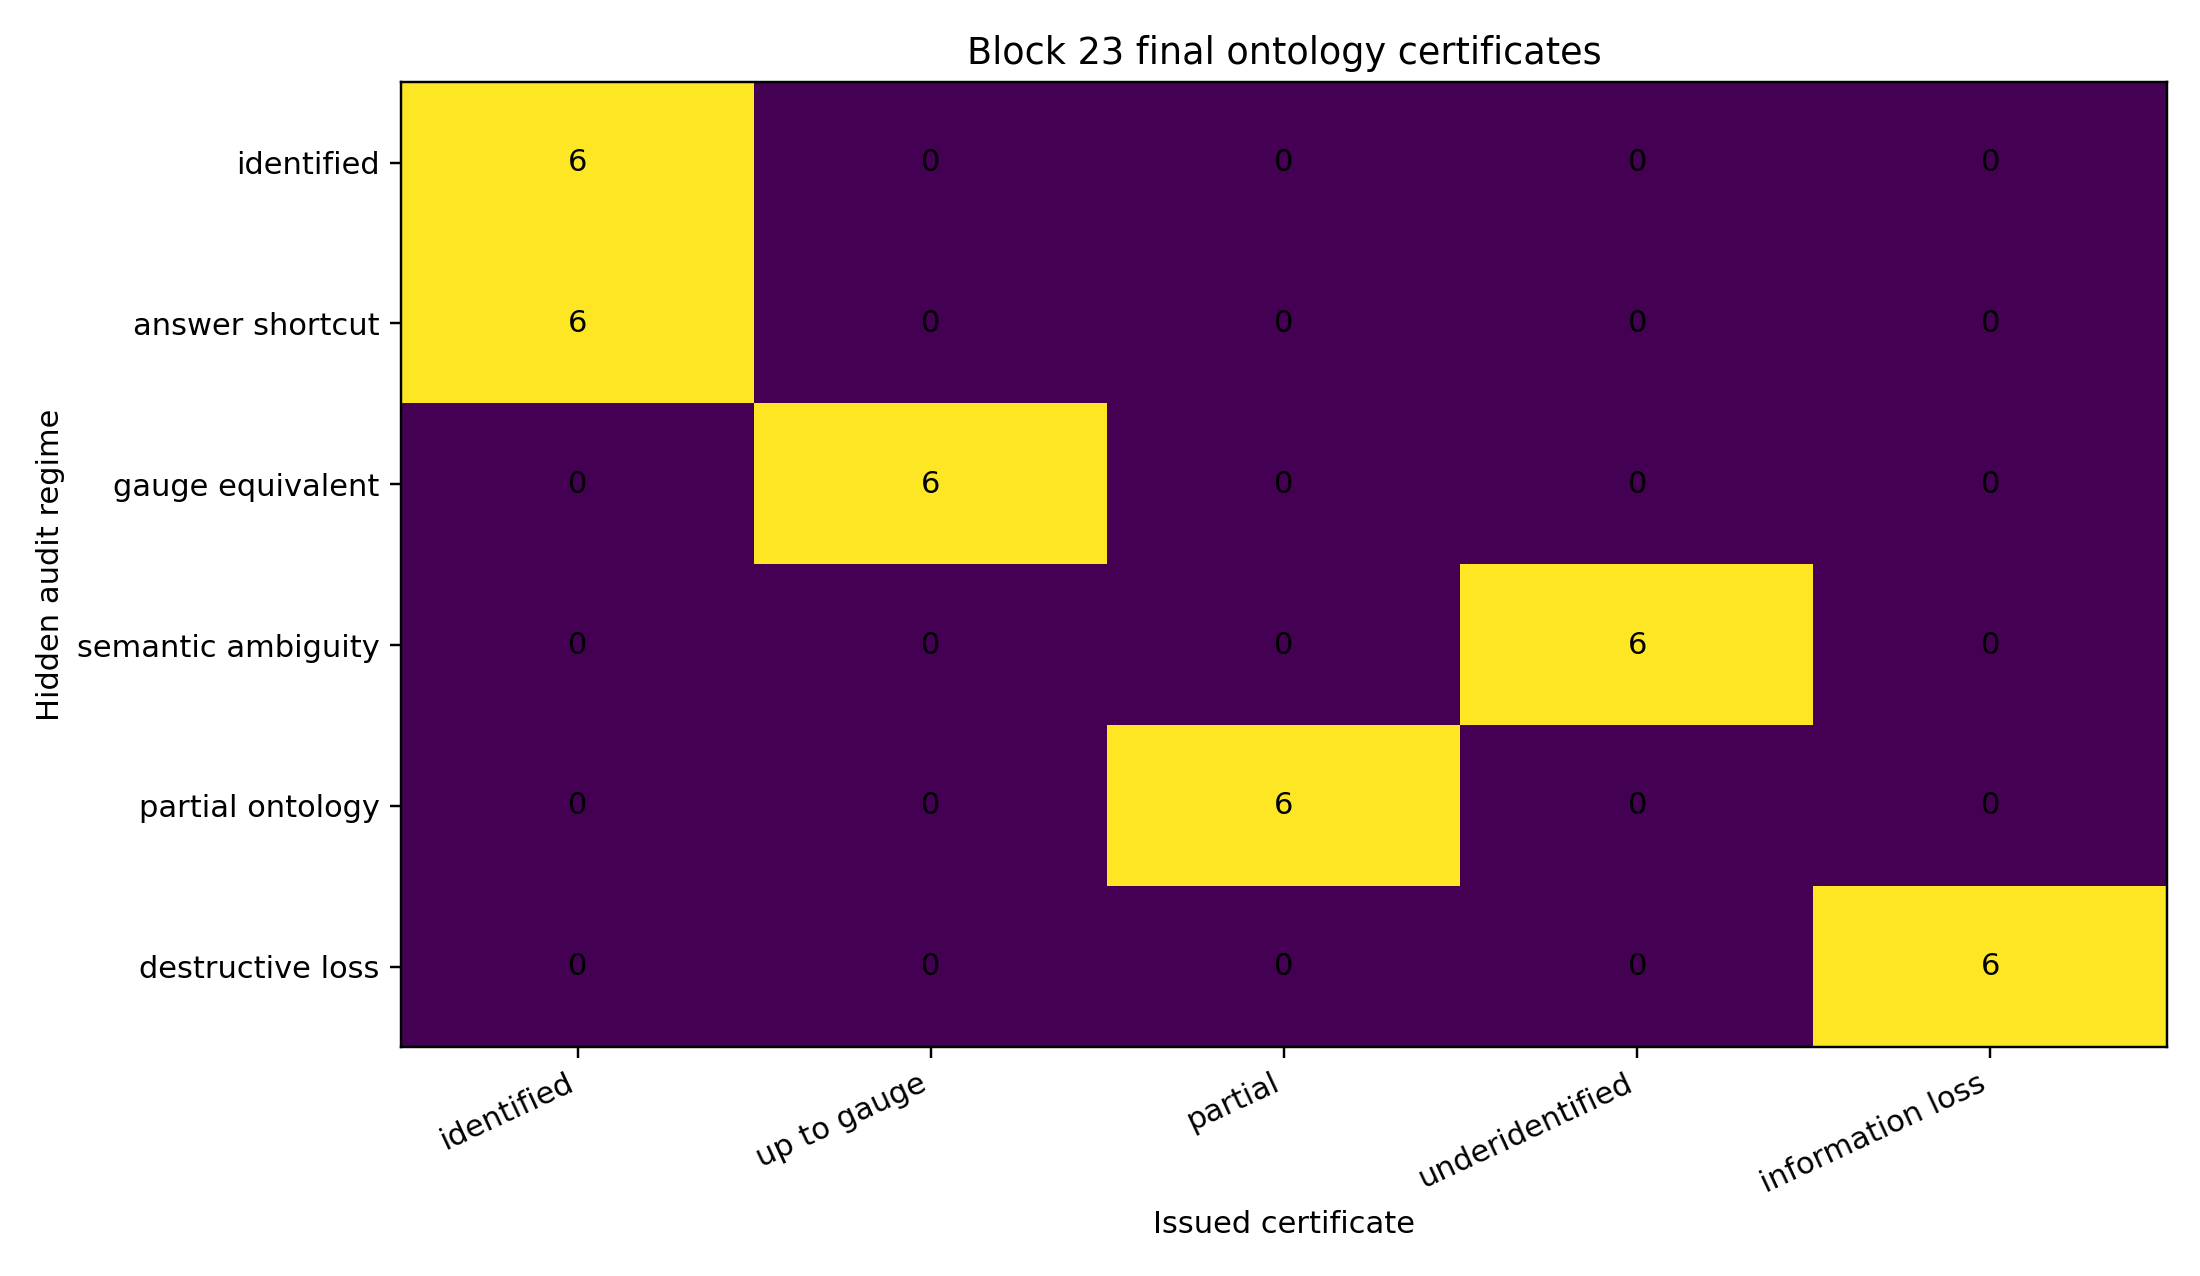
\includegraphics[width=0.92\textwidth]{block23_certificate_matrix.png}
\caption{Final hidden regime by issued ontology certificate.  The answer-shortcut regime remains identifiable only because the compiler rejects the one-dimensional answer code and selects a four-dimensional predictive quotient.}
\label{fig:b23-certificate-matrix}
\end{figure}

The selected constructions were:
\begin{itemize}
\item a rank-four predictive quotient for the identified and answer-shortcut regimes;
\item a rank-four intervention-response quotient for the gauge-equivalent and semantic-ambiguity regimes;
\item a rank-three predictive quotient for the partial regime;
\item no admitted quotient for destructive information loss.
\end{itemize}

\begin{figure}[H]
\centering
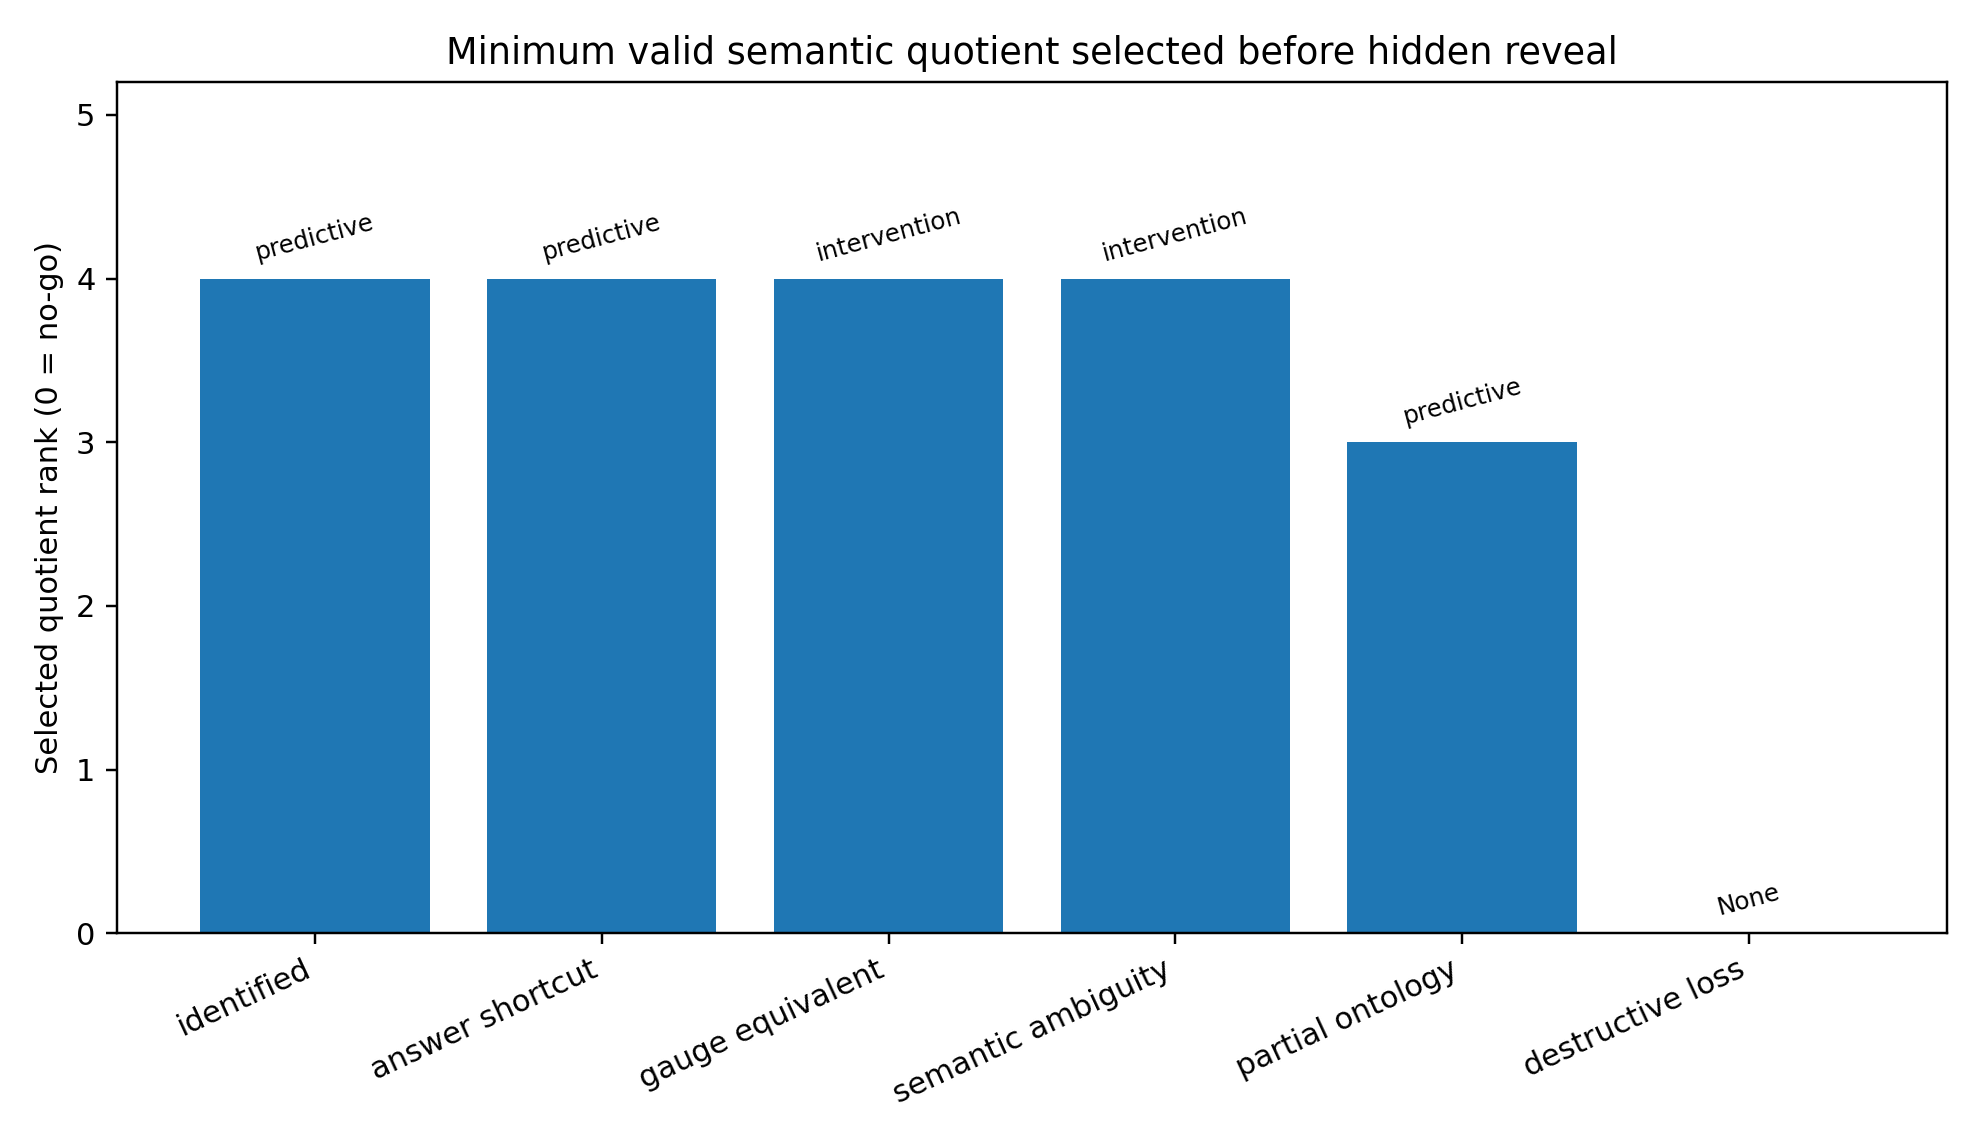
\includegraphics[width=0.88\textwidth]{block23_minimal_quotients.png}
\caption{Minimum valid quotient ranks and selected constructor classes.  Zero denotes a collision-grounded no-go rather than an empty semantic success.}
\label{fig:b23-minimal-quotients}
\end{figure}

\subsubsection{Answer-only negative control}

In the answer-shortcut episodes, the rank-one answer projection achieved held-out answer accuracy at least $0.881250$.  Nevertheless, its best future-consequence and intervention-effect scores were only
\begin{equation}
R^2_{\mathrm{future}}\leq0.313061,
\qquad
R^2_{\mathrm{intervention}}\leq0.357401.
\end{equation}
It failed every final construction decision.  This separates answer extraction from semantic-state recovery.

\subsubsection{Hidden semantic and gauge audit}

Across uniquely identified regimes, hidden semantic reconstruction is numerically exact in the released fixture.  In the gauge regime, minimum gauge-invariant $R^2$ is $0.995522$, while the minimum recovered semantic-subspace overlap is $0.991563$.  In the semantic-ambiguity regime, the minimum protected disagreement between two observationally equivalent orientations is $0.781682$.  Although either orientation is post-hoc decodable, the correct disposition remains underidentified.

The partial regime identifies three of four protected directions, giving coverage $0.75$.  The fourth direction is not assigned a fabricated value.  Every destructive episode contains $64$ exact collision pairs; the minimum disagreement in externally protected future consequences is $1.736704$.  The collision witness never receives a hidden intermediate semantic coordinate.

\subsubsection{Audit-only counterfactual packet patching}

After quotient commitment, a donor quotient replaces the selected packet in a new recurrent state.  The protected future and intervention consequences are recomputed through an audit-only runtime decoder rather than the probe used during construction.  The minimum selected-packet donor future $R^2$ is $0.983162$.  The maximum corresponding values for answer-only, PCA, and random controls are $-0.161100$, $-0.706230$, and $-0.703696$.

\begin{figure}[H]
\centering
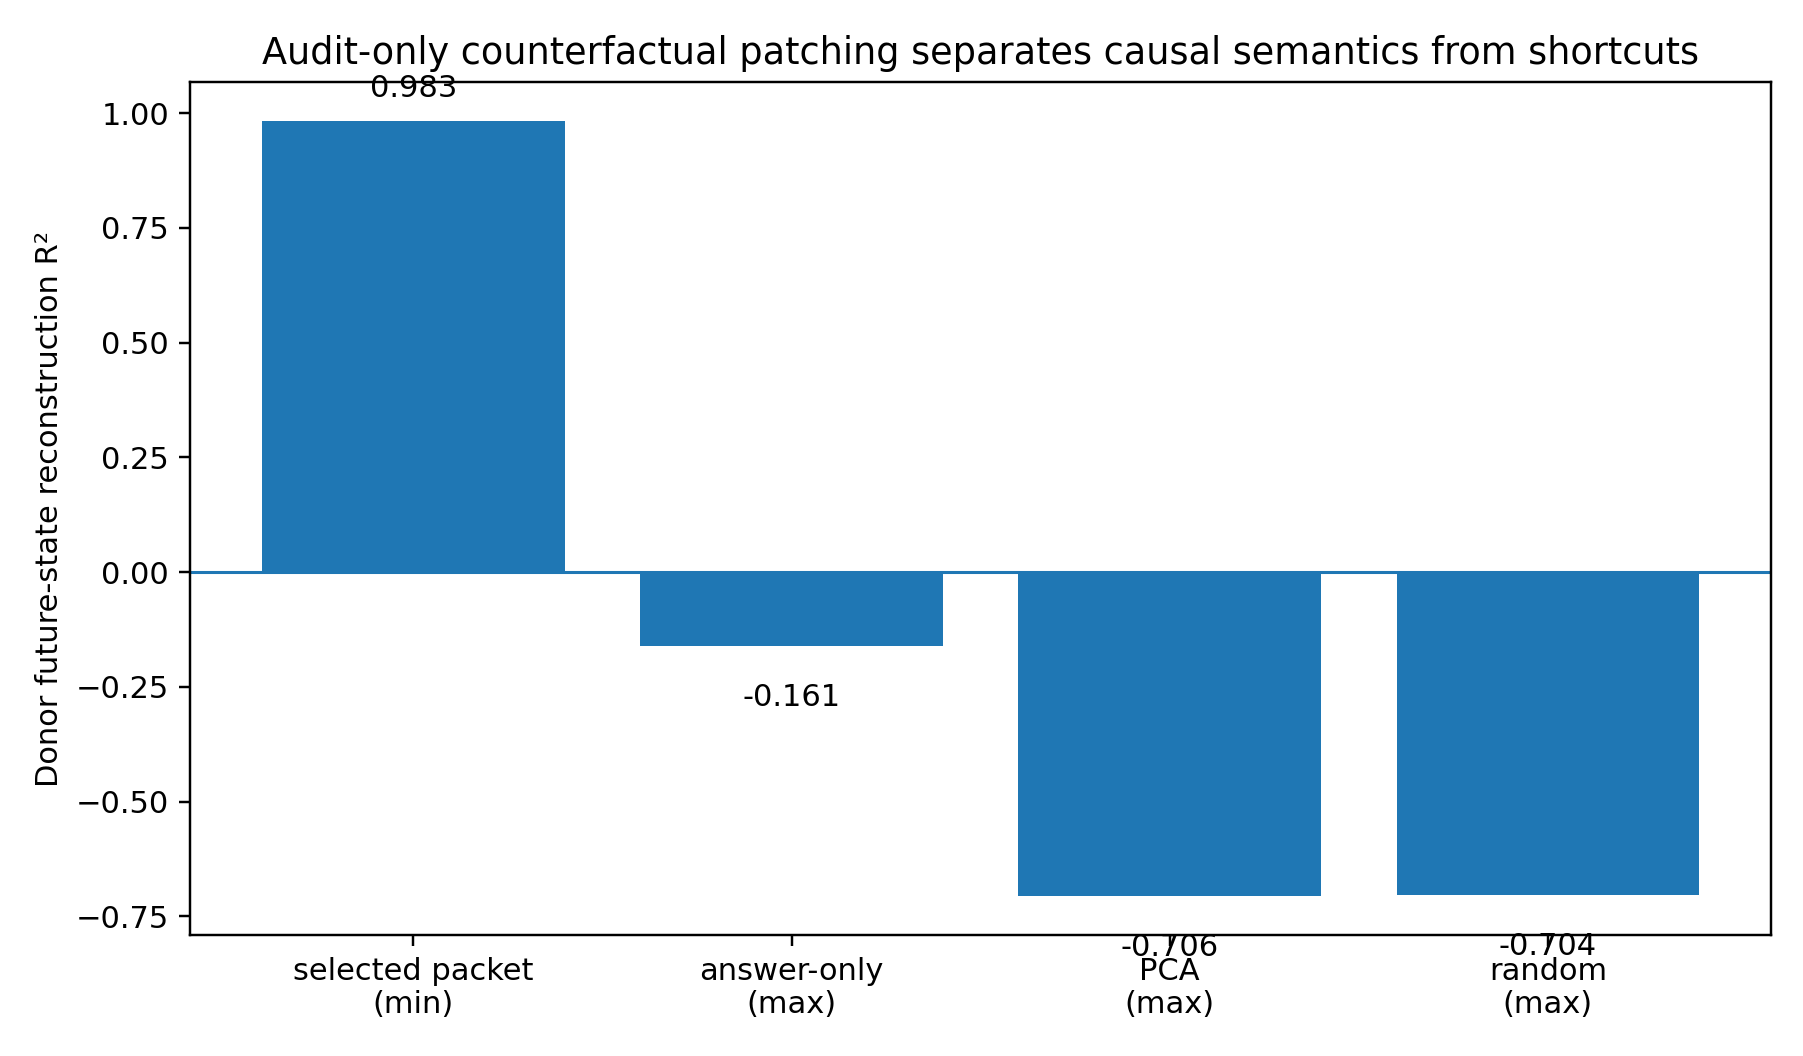
\includegraphics[width=0.82\textwidth]{block23_counterfactual_controls.png}
\caption{Counterfactual donor-packet controls.  Only the compiled quotient produces the predicted downstream future state in the identified and answer-shortcut regimes.}
\label{fig:b23-counterfactual-controls}
\end{figure}

\subsection{Finite realization theorem}

\begin{conditionaltheorem}[Block 23 finite endogenous semantic-witness growth]
Within the frozen Block 23 benchmark, assume that:
\begin{enumerate}
\item the visible compiler interface excludes hidden intermediate semantics and hidden regime labels;
\item construction and hidden witness supports are separated;
\item the candidate grammar, ranks, thresholds, seeds, and method priority are sealed before final hidden audit;
\item both recurrent systems share protected consequences but use independently generated gauges and nuisance processes;
\item the visible gates in \cref{eq:b23-visible-gates} are replayed exactly;
\item the hidden certificate rules distinguish unique identification, gauge equivalence, partiality, protected ambiguity, and exact semantic collision;
\item the thirty-six final results and their matrix digests reproduce the released receipt;
\item the answer-only, PCA, random-packet, alternative-orientation, and collision controls retain their declared interpretations.
\end{enumerate}
Then the released edge is a finite lineage-generated instance of endogenous semantic-witness growth: the compiler constructs a minimum-rank causal-predictive quotient without gold intermediate coordinates, and the witness assigns the appropriate unique, gauge, partial, underidentified, or information-loss certificate.
\end{conditionaltheorem}

\begin{proof}
Items 1 through 3 provide evidence separation and chronology.  Items 4 and 5 establish that the selected quotient is based on protected future and intervention behavior rather than one coordinate system or one answer label.  Item 6 prevents post-hoc decodability from being confused with unique identification and prevents destructive collisions from being treated as ordinary model error.  Item 7 supplies the finite replay certificate.  Item 8 rules out the principal answer-shortcut, variance, random-subspace, arbitrary-gauge, and correlation-based reconstruction explanations inside the released fixture.
\end{proof}

\subsection{External multimode Coconut pilot}

The package also freezes a first real-model audit target from Dilgren and Wiegreffe's multimode latent-reasoning release~\cite{DILGREN2026}.  The target checkpoint uses GPT-2 on PrOntoQA and supports latent, verbalized-chain-of-thought, and direct-answer modes in one trained model.  Its public Coconut wrapper replaces each latent-token embedding by the preceding final hidden state.  The wrapper returns the completed input-embedding tensor, making the exact reinjected latent states directly capturable.

The Block 23 adapter does not rely on an ordinary activation hook as a substitute for the recurrence.  It identifies the latent-token positions, extracts the embeddings actually written there, and evaluates an externally supplied trace by replacing those positions in a deterministic one-shot recomputation.  The intervention language includes:
\begin{enumerate}
\item exact own-trace replay;
\item zero trace and prefix truncation;
\item frozen step permutation;
\item norm- or covariance-matched replacement;
\item same-answer, different-proof transplantation;
\item semantic-twin transplantation by consistent entity and predicate renaming.
\end{enumerate}

The source lock commits the upstream repository at
\begin{verbatim}
32f413d8d55239d9bc54bb6b6ec37b0630891ed4
\end{verbatim}
and records the Git blob identities of the Coconut wrapper, multimode adapter, base interface, and PrOntoQA test data.  The checkpoint digest is intentionally left unset until the actual local file is acquired; the runner computes and commits its SHA-256 before any final audit.

\subsubsection{Adapter fixture}

A deterministic fake runtime tests protocol plumbing but is excluded from the external empirical claim.  Across $72$ fixture tasks it yields exact replay error zero, mean zero-trace cost $0.533811$, permutation cost $0.038959$, norm-matched-noise cost $0.459498$, same-answer different-program transplant cost $0.311093$, and semantic-twin transplant cost zero.

\subsubsection{External execution status}

The release environment had CPU-only PyTorch, no \texttt{transformers} installation, no source checkout, and no checkpoint file.  The canonical external status is therefore
\begin{verbatim}
ADAPTER_VALIDATED_REAL_EXECUTION_BLOCKED
\end{verbatim}
with \texttt{real\_checkpoint\_executed=false}.  No external checkpoint loss, causal effect, semantic quotient, or interpretability certificate is reported.

\begin{warning}[No substitution of fixture evidence]
Passing the fake-runtime protocol tests does not imply that the third-party checkpoint replays exactly, uses its latent tokens, contains procedure-specific information, or admits an identifiable semantic quotient.  Those questions remain empirical.
\end{warning}

\subsection{Reproducibility and claim boundary}

The canonical finite result receipt is
\begin{verbatim}
213bcf9fbf62b797f9903d9e05e84e5a4036bb02c927723a4570fa44e2c674ce
\end{verbatim}
and the adapter-fixture receipt is
\begin{verbatim}
e447e082f3befe5b7b6bb0254464c4cb1402684a0c93e3022579439be6f62664
\end{verbatim}
The released tests cover visible-interface isolation, all final certificates, answer-shortcut rejection, counterfactual packet controls, collision no-go, external causal-audit plumbing, gold-free discovery, and fail-closed preflight.

Block 23 establishes neither unrestricted ontology discovery nor interpretation of natural-language reasoning.  It does not show that every latent state has a unique verbal meaning.  It establishes a finite architecture in which semantic claims are grounded in protected future and intervention behavior, assigned only after witness separation, and allowed to terminate in gauge ambiguity, partiality, underidentification, or information-loss no-go.

The next threshold is empirical.  The source-locked Coconut checkpoint should be run on a family-grouped PrOntoQA audit.  Exact replay must pass before any causal claim.  A quotient should then be constructed without proof steps, sealed, and only afterward compared with withheld formal proof chains and counterfactual premise edits.  A second threshold would transport any validated quotient to the corresponding CODI checkpoint without exact task-level pairing.

\begin{thebibliography}{9}\footnotesize
\bibitem{DILGREN2026}
Connor Dilgren and Sarah Wiegreffe,
\emph{Are Latent Reasoning Models Easily Interpretable?},
arXiv:2604.04902, 2026.
\bibitem{SRICB22}
Komorebi P.,
\emph{SRIC v2.3 Block 22 Correspondence-Free Neuralese Transport from Intervention Orbits},
reference implementation and cumulative theory draft, 2026.
\end{thebibliography}
\end{document}
